\section{Descrizione e motivazioni delle tecnologie adottate }
In questa sezione vengono presentate le tecnologie adottate per l’implementazione delle componenti client e server del sistema.
Inoltre, vengono descritte le architetture specifiche utilizzate nel back-end, in relazione alle tecnologie impiegate, e quelle adottate nel front-end.

\subsection{Tecnologie e architettura backend}
L'architettura del nostro server è stata progettata per rispondere alle esigenze richieste dal cliente, dove è stata prioritizzata la velocità di sviluppo e deployment senza sacrificare robustezza e sicurezza. Abbiamo adottato un'architettura \textbf{monolitica} basata su una struttura a livelli, che facilita la separazione delle responsabilità e garantisce una maggiore manutenibilità nel tempo. La scelta di un'architettura monolitica si giustifica con la necessità di ridurre la complessità iniziale e non rallentare lo sviluppo, mantenendo comunque una struttura modulare che potrà essere facilmente evoluta nel tempo, ad esempio, trasformando parti del sistema in microservizi qualora il progetto dovesse espandersi in futuro.
\\
Le tecnologie selezionate per lo sviluppo del backend sono state scelte in base a una combinazione di familiarità e facilità d'uso, con l'obiettivo di accelerare il processo di implementazione e garantire al contempo solidità e qualità del codice.
\\
Il back-end è stato sviluppato utilizzando \textbf{Spring Boot}, abbiamo optato per questo framework grazie alle sue numerose configurazioni predefinite e utili estensioni come \textbf{Lombok}, che ci permettono di concentrarci sulla logica di business anziché su complesse configurazioni di sistema o codice ripetuto. Spring Boot consente di avviare rapidamente un'applicazione web robusta e scalabile.
esso sono state integrate diverse tecnologie complementari, tra cui:

\begin{itemize}
	\item \textbf{Hibernate}: Per la gestione della persistenza, Hibernate si rivela una scelta efficace, in quanto astrae le operazioni di accesso al database e riduce significativamente il lavoro manuale nella scrittura di query SQL. Questo approccio rende il codice più leggibile e facilmente mantenibile.
	
	\item \textbf{Spring Security e JWT (JSON Web Token)}: Per garantire un'autenticazione stateless e sicura, abbiamo deciso di utilizzare i JWT. Questa soluzione permette di gestire le sessioni degli utenti in maniera efficiente, differenziando eventuali ruoli o permessi e riducendo il carico sul server.
	
	\item \textbf{Jackson}: È uno strumento potente per serializzare e deserializzare oggetti Java in \textbf{JSON} e viceversa.
	Quando si utilizza l’annotazione \colorbox{lightgray}{@RestController} o \colorbox{lightgray}{@ResponseBody}, Spring Boot restituisce automaticamente le risposte in formato JSON senza necessità di configurazioni aggiuntive.
	
	\item \textbf{Swagger}: L’adozione di Swagger per la documentazione delle REST API agevola notevolmente il testing e la verifica degli endpoint, creando al contempo una documentazione ricca di informazioni utili per condividere informazioni critiche.
\end{itemize}

Il back-end del sistema segue il pattern architetturale \textbf{MVC (Model-View-Controller)}, nativamente supportato dal framework \textbf{Spring Boot}.
Nel nostro caso, il \textbf{Model} è rappresentato dalle entità e dalla logica di business implementata nei servizi; il \textbf{Controller} è costituito dai componenti RESTful che gestiscono e mappano le richieste HTTP.
La \textbf{View} non è gestita all’interno del back-end, poiché l’applicazione svolge il ruolo di \textbf{API REST}, restituendo risposte in formato JSON al client, che si occupa della rappresentazione dei dati.
Questo approccio garantisce una chiara \textbf{separazione delle responsabilità}, migliorando la \textbf{modularità} e la \textbf{manutenibilità} del sistema.
\\ \\
Di seguito viene riportato uno schema del design utilizzato del backend

\begin{figure}[H]
	\centering
	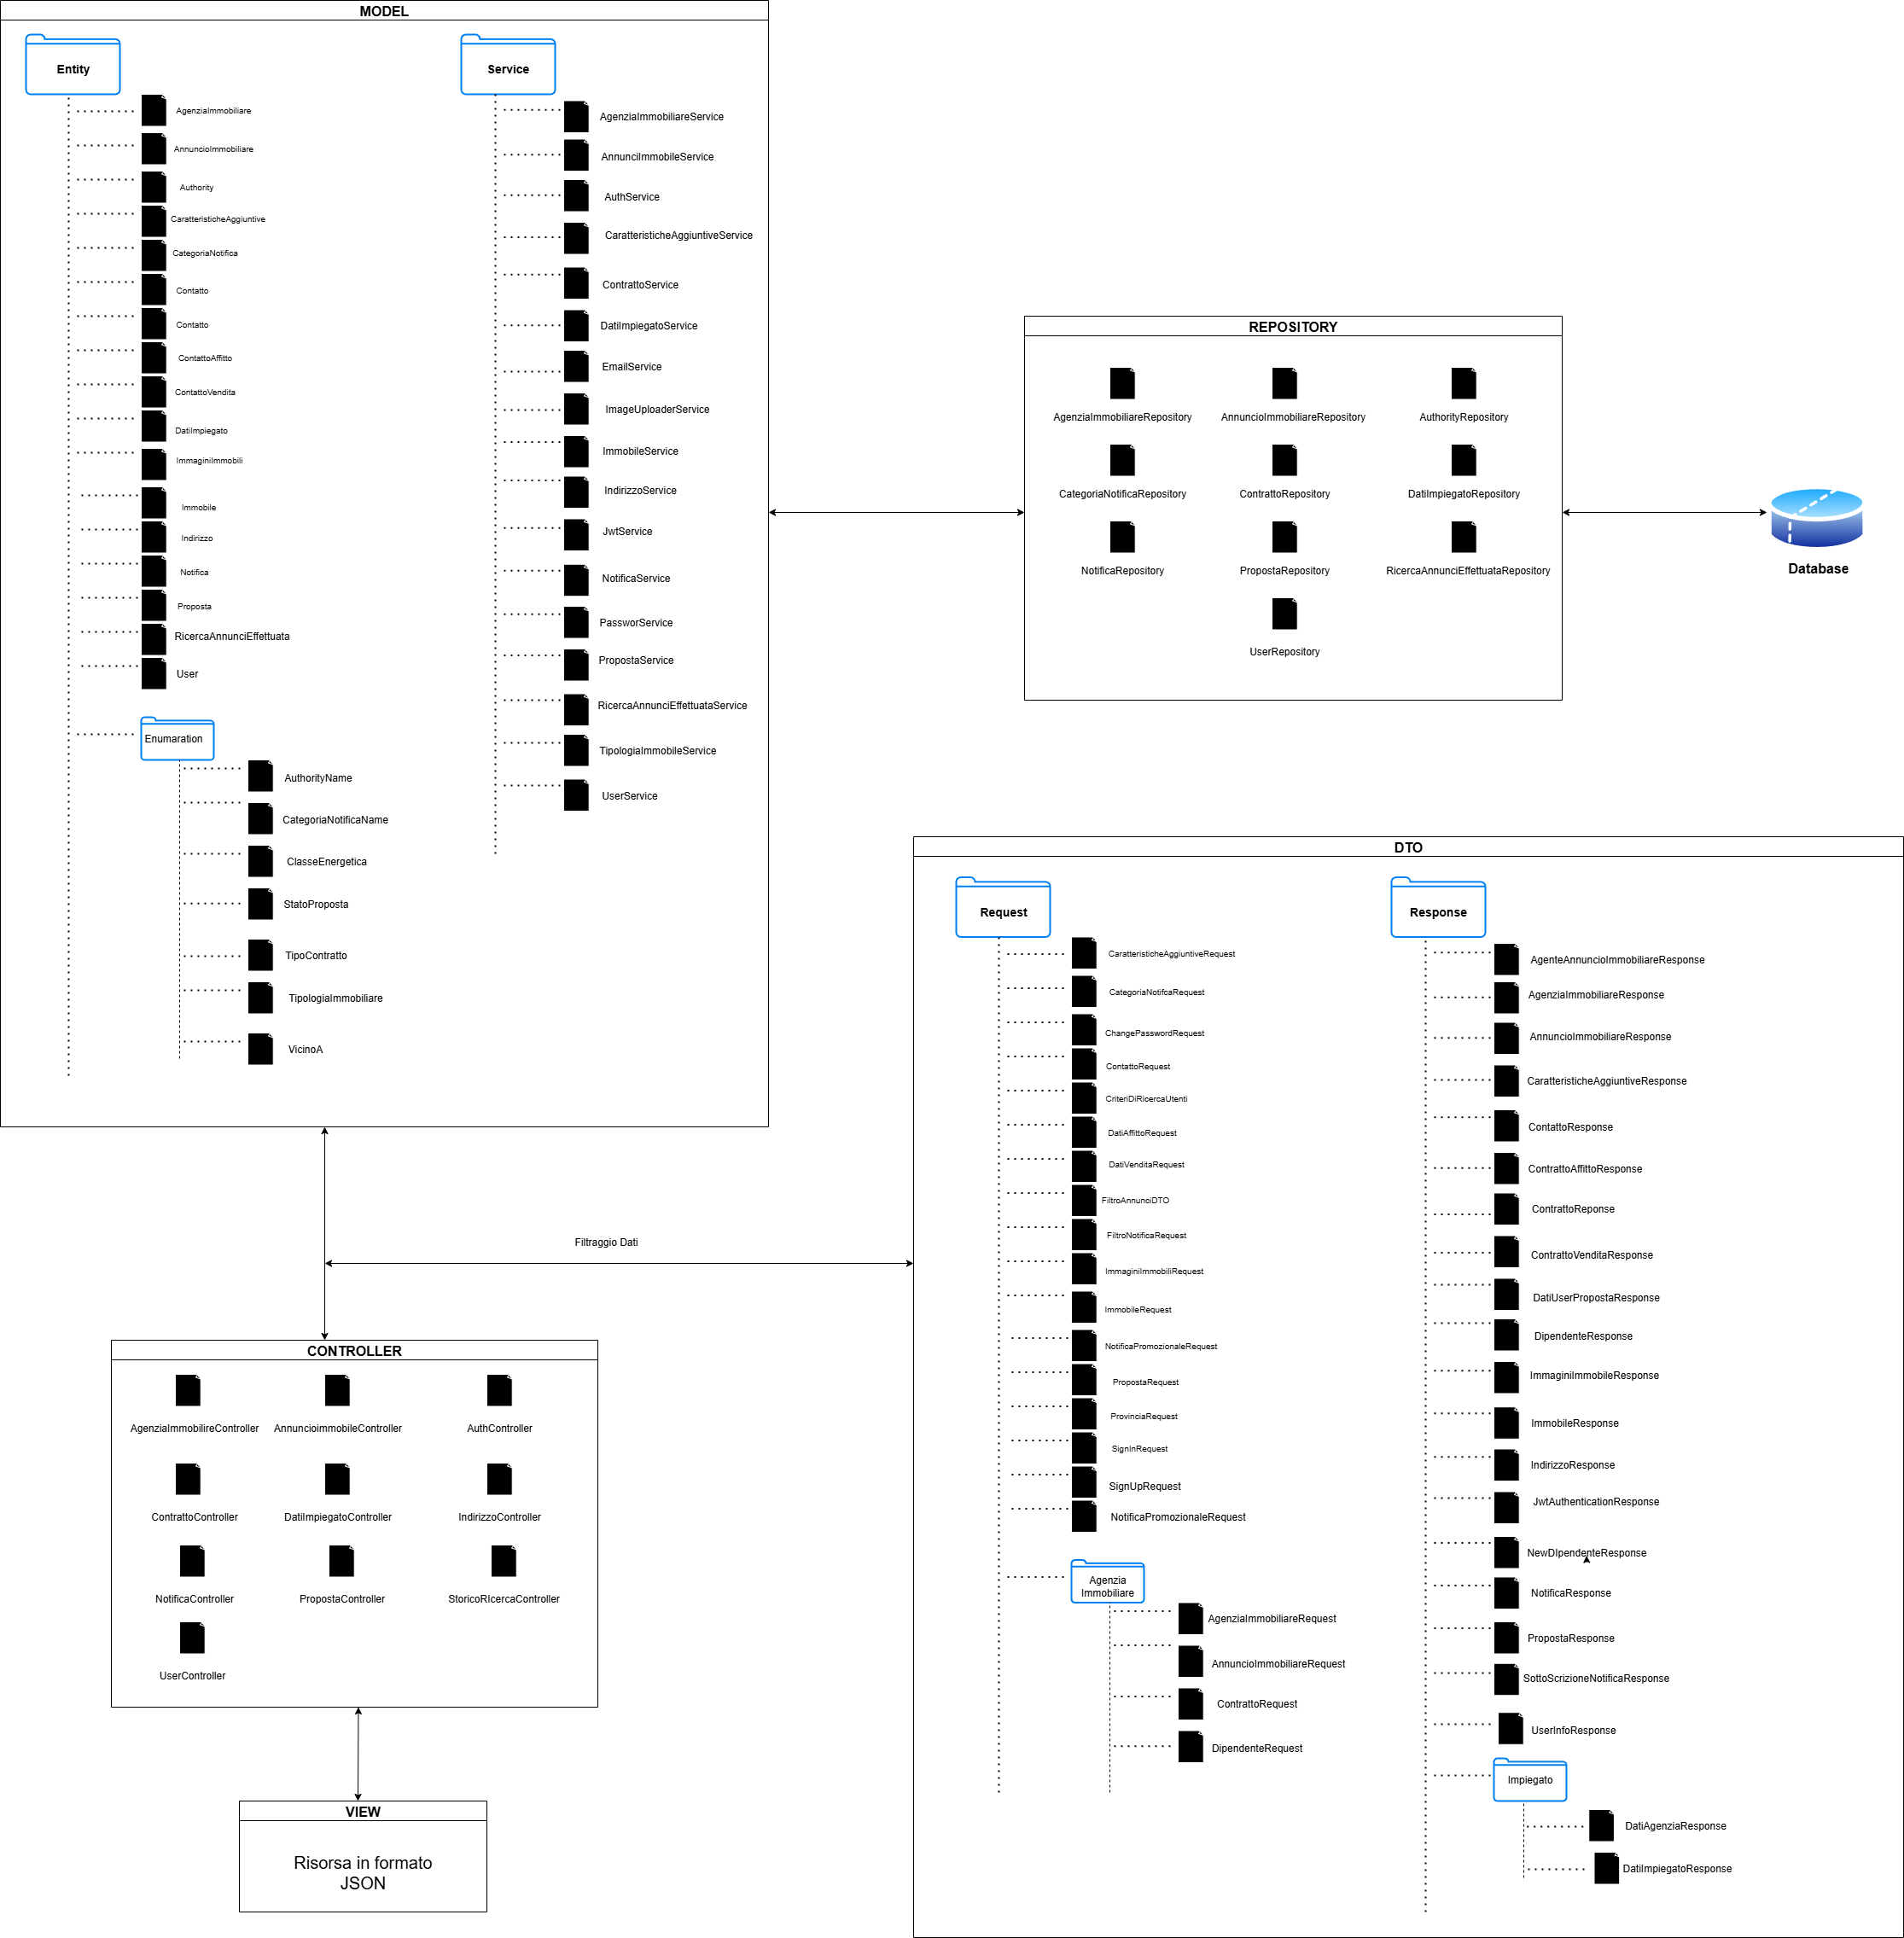
\includegraphics[width=1\linewidth]{Immagini/Schema backend.png}
	\caption[schema backend]{Schema sintetico dell'architettura del backend}
\end{figure}

\begin{itemize}
	
	\item \textbf{MODEL}: Il Modello rappresenta i dati e la logica di business dell’applicazione, indipendentemente da come questi dati vengano visualizzati. In un’architettura MVC, il modello non deve dipendere dalle viste né dai controller, ma deve fornire metodi che consentano ai \textbf{controller} di manipolare i dati in risposta alle richieste dell’utente. Nel contesto del
	nostro sistema, il package \textbf{Service} all’interno del Model offre i metodi necessari per la 22 manipolazione dei dati relativi alle entità. Queste entità, grazie alle \textbf{funzionalità di Spring Boot}, sono mappate automaticamente alle relative tabelle nel database, facilitando l’interazione con i dati persistenti. L’accesso ai dati avviene tramite il \textbf{repository}, che permette di recuperare le informazioni direttamente dal database.
	
	\item \textbf{CONTROLLER}:  Il Controller svolge un ruolo fondamentale nell’architettura MVC come \textbf{ponte tra il Model e la View}. In particolare, gestisce le interazioni dell’utente, elabora le richieste e aggiorna sia il Model che la View in base alle azioni dell’utente.
	Quando un utente interagisce con l’interfaccia (la View), il Controller riceve l’input, elabora i dati (eventualmente tramite il Model, che contiene la logica di business) e quindi
	aggiorna la View per riflettere i cambiamenti dello stato. Nel nostro sistema, che segue l’architettura \textbf{RESTful API}, l’input dell’utente è rappresentato dalle richieste \textbf{HTTP (come POST, GET, PUT, DELETE)}. Ogni Controller gestisce le richieste relative a una specifica entità (ad esempio, UserController, AgenziaImmobiliareController, ecc.) e quindi si occupa di ricevere e rispondere a queste richieste. Una particolarità del nostro sistema è l’uso di \textbf{DTO (Data Transfer Object)}, che funge da \textbf{strato di filtraggio} tra la logica di business (Model) e le risposte al client. Le DTO vengono utilizzate per limitare i dati che vengono passati nelle richieste e nelle risposte. In altre parole, quando un client invia una richiesta al Controller o quando il Controller restituisce una risposta, la DTO permette di selezionare solo le informazioni necessarie, evitando di esporre direttamente l’intera entità. Questo approccio migliora la \textbf{sicurezza} e l’\textbf{efficienza}, poiché impedisce di passare dati non necessari e riduce il rischio di esposizione di informazioni sensibili. Per esempio, se un’entità Utente ha campi come id, nome, email, password, il Controller potrebbe rispondere con una DTO che include solo i campi nome ed email, evitando di restituire campi sensibili come la password. In questo modo, solo le informazioni realmente necessarie per il client vengono trasmesse.
	
	\item \textbf{VIEW}: La View è responsabile della \textbf{rappresentazione grafica dei dati} e dell’interfaccia utente. Poiché il nostro back-end è un’architettura \textbf{API RESTful}, la View viene gestita interamente dal client.
	
\end{itemize}

Il sistema include ulteriori pacchetti che contengono classi di configurazioni o classi di ausilio: 

\begin{itemize}
	
	\item In \textbf{config} troviamo le classi necessari per la configurazione del framework e la gestione della sicurezza, come l’autenticazione, essenziale per garantire l’accesso controllato agli end-point e il corretto esito delle risposte
	HTTP. Ad esempio, gli end-point che iniziano con \colorbox{lightgray}{/pb} sono configurati come accessibili liberamente, senza necessità di autenticazione. Questa impostazione viene definita nel file \textbf{SecurityConfiguration}, situato all’interno.
	
	\item In \textbf{exception} ci sono le classi che estendono RunTimeException.
	Ogni eccezione personalizzata rappresenta uno specifico stato di errore HTTP restituito nella risposta. La classe \colorbox{lightgray}{ExceptionManagement} gestisce tutte le eccezioni personalizzate, mappandole sul corretto codice di errore HTTP al momento del loro lancio.
	
	\item In \textbf{utils} contiene classi che offrono metodi statici di utilità riutilizzabili dai componenti del livello service. 
	In particolare \colorbox{lightgray}{getUserCurrent()} della classe UserContex, ampiamente utilizzato per ottenere l’utente che ha effettuato una richiesta HTTP tramite il contesto di sicurezza di Spring (SecurityContext).
	
	\item Infine rimangono i package \textbf{factory} e \textbf{strategy} contengono le classi di supporto ai service responsabili dell’invio di notifiche agli utenti, generando dinamicamente il contenuto in base alla categoria della notifica. Tale esigenza è stata risolta applicando il \textbf{pattern Factory Method}, che prevede la definizione di una \textbf{interfaccia comune} e di \textbf{classi factory specifiche} in grado di restituire l’istanza più appropriata in base al contesto.
	In combinazione, il \textbf{pattern Strategy} consente di definire comportamenti diversi per la generazione del contenuto della notifica, migliorando flessibilità e manutenibilità del sistema.
	
\end{itemize}
 
